\documentclass{article}

\usepackage{makecell, graphicx}
\graphicspath{ {./images/} }

\title{Ch. 31 CW (Cont'd)}
\author{Principles of Macroeconomics}
\date{\today}

\begin{document}

\maketitle

\section*{Instructions} Please do the following problems on another sheet of paper and fully justify your answers.

\section*{Problems}

\begin{enumerate}

\item How will the following events affect the demand for money? In each case, specify whether there is a shift of the money demand curve or a movement along the money demand curve.

	\begin{enumerate}
	
	\item Thanksgiving arrives and, with it, the beginning of the holiday shopping season.
	
	\item McDonald's and other fast-food restaurants begin to accept credit cards.
	
	\item The Fed engages in an open-market purchase of U.S. Treasury bills.
	
	\end{enumerate}
	
\item The accompanying table shows the annual growth of the money supply and nominal GDP in Japan during the early 2000s. What must have been happening to velocity during this time? 

	\begin{tabular}{c | c | c }
	\textbf{Year} & \makecell{\textbf{Money Supply}\\\textbf{Growth}} & \makecell{\textbf{Nominal GDP}\\\textbf{Growth}} \\
	\hline
	2000 & 8.2\% & 2.9\% \\
	2001 & 8.5\% & 0.4\% \\
	2002 & 27.6\% & -0.5\% \\
	2003 & 8.2\% & 2.5\%
	\end{tabular}
	
\item In the economy of Eastlandia, the money market is initially in equilibrium when the economy begins to slide into a recession (real GDP shrinks). 

	\begin{enumerate}
	
	\item Assuming the velocity of money is constant, explain what happens to the price level if the central bank keeps the money supply constant. 
	
	\item If the central bank wants to maintain a constant price level, how should it change the money supply?
	
	\end{enumerate}
	
\item Boris Borrower and Lynn Lender agree that Lynn will lend Boris \$10,000 and that Boris will repay the \$10,000 with interest in one year. They agree to a nominal interest rate of 8\%, reflecting a real interest rate of 3\% on the loan and a commonly shared expected inflation rate of 5\% over the next year.

	\begin{enumerate}
	
	\item If the inflation rate is actually 4\% over the next year, how does that lower-than-expected inflation rate affect Boris and Lynn? Who is better off?
	
	\item If the actual inflation rate is 7\% over the next year, how does that affect Boris and Lynn? Who is better off?
	
	\end{enumerate}
	
\item In the following examples, is inflation creating winners and losers at no net cost to the economy or is inflation imposing a net cost on the economy? If a net cost is being imposed, which type of cost is involved?

	\begin{enumerate}
	
	\item When inflation is expected to be high, workers get paid more frequently and make more trips to the bank.
	
%	\item Lanwei is reimbursed by her company for her work-related travel expenses. Sometimes, however, the company takes a long time to reimburse her. So when inflation is high, she is less willing to travel for her job.
	
	\item Hector Homeowner has a mortgage with a fixed nominal 6\% interest rate that he took out five years ago. Over the years, the inflation rate has crept up unexpectedly to its present level of 7\%.
	
	\item In response to unexpectedly high inflation, the manager of Cozy Cottages of Cape Cod must reprint and resend expensive color brochures correcting the price of rentals this season.
	
	\end{enumerate}
	
\item The accompanying diagram shows mortgage interest rates and inflation during 1990-2005 in the economy of Albernia. When would home mortgages have been especially attractive and why?
	
	\begin{center}
	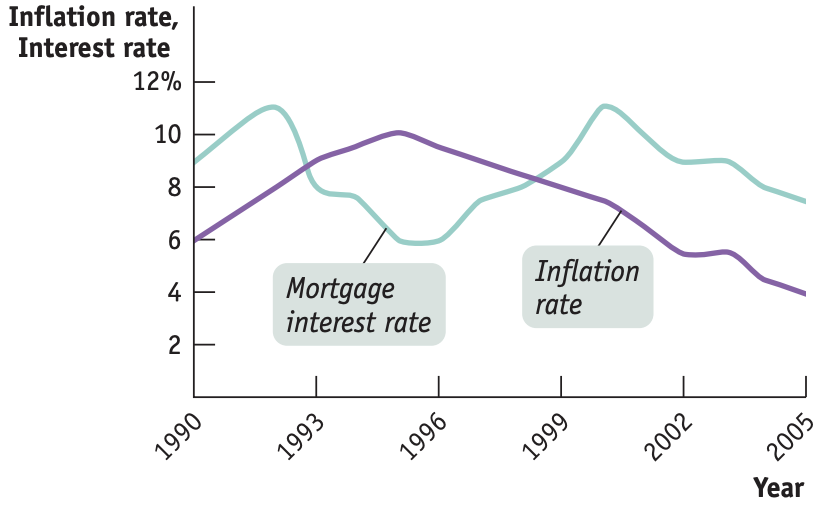
\includegraphics[width = 0.75\textwidth]{cw2_q5}
	\end{center}

\end{enumerate}

\end{document}